\section{Game Development}
\label{chap:game_development}
The first three months of working with this project were primarily dedicated to developing Hover. The following sections will explain the development process and how the software architecture was designed.

\subsection{Development Process}
\begin{wrapfigure}{r}{0.45\textwidth}
    \vspace*{-1\baselineskip}
    \centering
    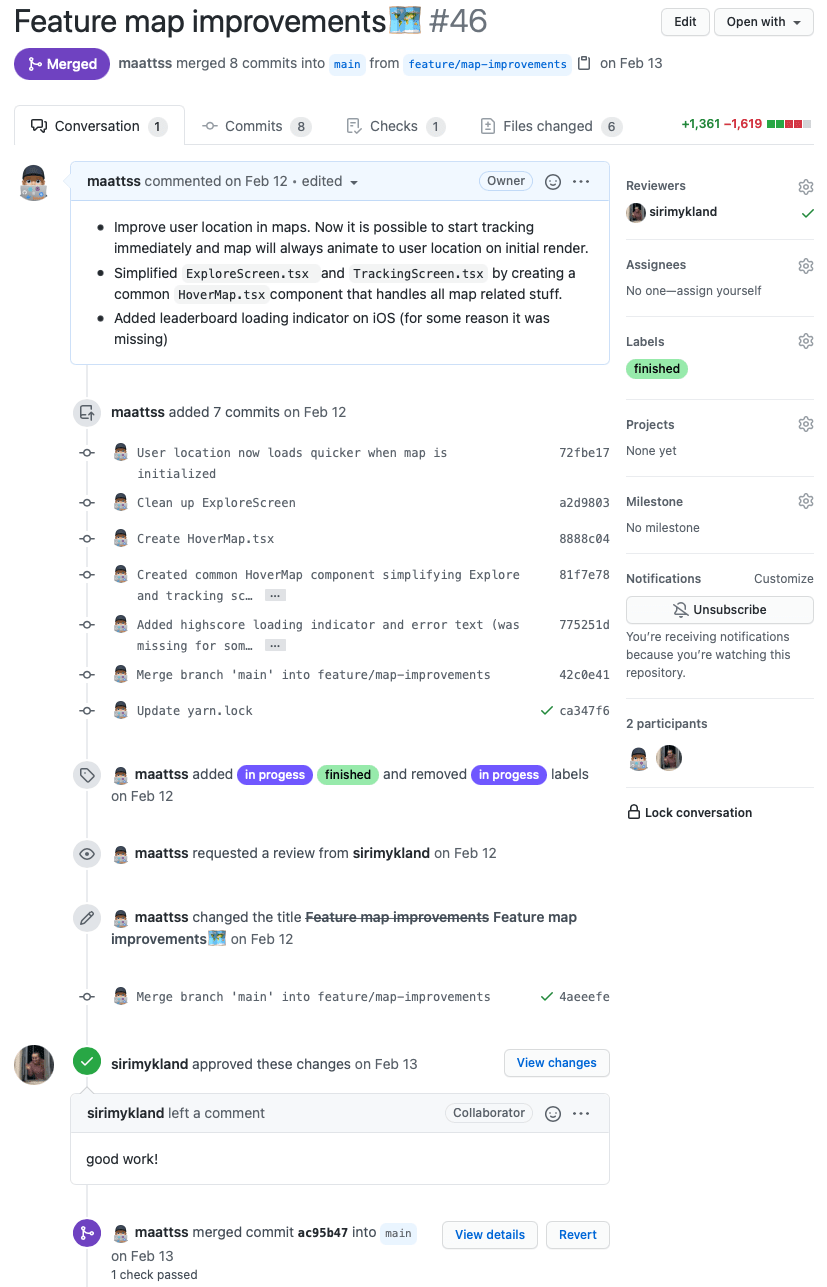
\includegraphics[width=0.35\textwidth]{Images/GameDevelopment/GithubPR.png}
    \caption{Typical pull request on Github from the development process.}
    \label{fig:github_pr}
\end{wrapfigure}

The first step in the development process was to set up code repositories, choose tools and agree on conventions. We used Git and Github as our version control system and collaboration tool. Conventions and other development information, such as setup and deployment processes, were stored in a \href{https://github.com/maattss/hover/wiki}{Wiki} in our repository on Github. To ensure that the code conventions were easy to follow, we utilized a linter in our editor and added a continuous integration check on Github. Additionally, we used pull requests and code reviews to catch errors, potential improvement possibilities and make sure both of us understood the code. Figure \ref{fig:github_pr} shows a screenshot from one of many completed pull requests during the development phase.

After conventions and tools had been settled, the next step was to plan how the game should be implemented and which features we should prioritize. The functional requirements described in Chapter \ref{chap:requirements} was used as the foundation for creating development tasks. To keep track of the tasks during the agile development process, we utilized a Kanban board. Figure \ref{fig:trello_board} shows a screenshot from the board during the development period. The tasks are categorized depending on their priority, and the ones up next are found in the “committed” list. The Kanban board made it easier for us to organize and keep track of all the tasks and remove possible uncertainty of what the other person was doing. In addition to the Kanban board, we had daily standups and discussions to keep the other person up to date on the task progress and potential problems or other hiccups. Because of the Covid-19 situation, we were sometimes forced to work remotely, collaborating using remote communication tools. The board and daily discussion showed their value in these periods.

\begin{figure}[H]
    \centering
    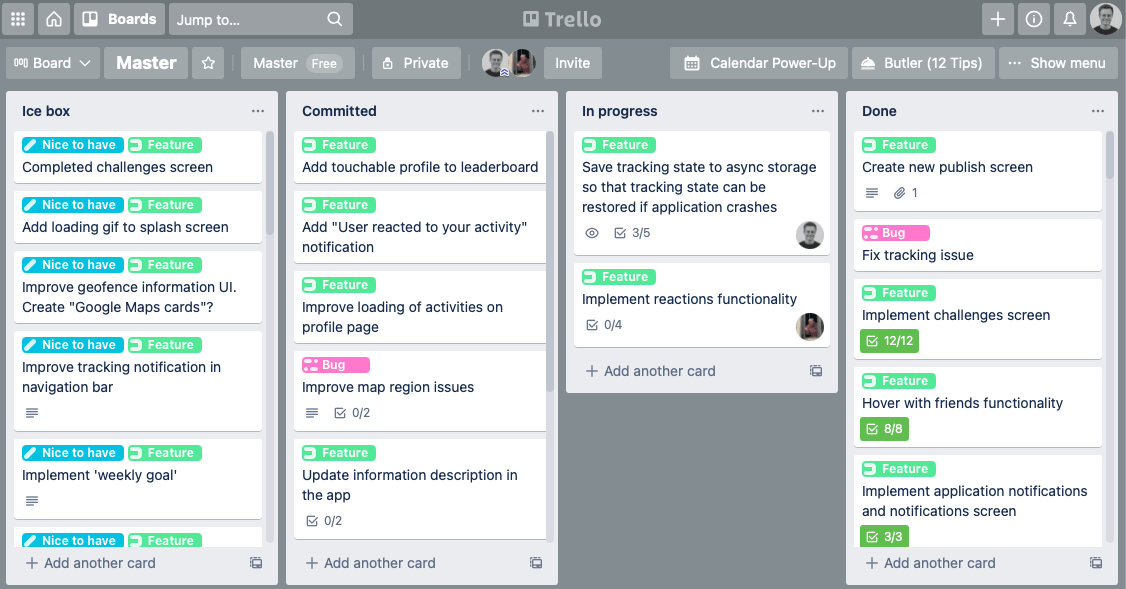
\includegraphics[width=0.95\textwidth]{Images/GameDevelopment/TrelloBoard.png}
    \caption{Kanban board from the development process.}
    \label{fig:trello_board}
\end{figure}

As in every development process, we tried to prevent unwanted bugs. Various best practices, such as keeping entities small and decreasing cognitive complexity, were used to improve code quality. In addition to this, we let selected friends and family that were not supposed to be a part of the test group, try the application during the development process. Continuous testing was an effective way to clear bugs and other issues that we had not experienced ourselves. We also got some other general feedback that helped improve the application from these people. 

Testing of the code was not implemented in this project. We had a discussion early on whether or not to include it. The decision became that it was not worth the effort since the goal of this development was to create a working prototype and not a full-fledged application. The focus was to implement as many features and game elements as possible during the limited time we had available.

The development period resulted in a working implementation of the game Hover deployed to App Store and Google Play. The process took approximately three months of full-time work with around 36500 lines of code produced and above 100 pull requests completed.

\subsection{Software Architecture}
Designing the software architecture is a crucial phase in the development of every modern system. In this section, a brief overview of the architecture of Hover will be given. We will not go into details of how the specific parts are developed. However, since all code is open-source, interested readers can dive deeper into how the system is structured by visiting repositories for the \href{https://github.com/maattss/hover}{mobile application} and the supporting \href{https://github.com/maattss/hover-functions}{backend} on Github.

As illustrated in Figure \ref{fig:architecture_overview}, the system consists of four main parts: the application, a Hasura storage solution, the Firebase backend, and Expo for handling notifications and OTA updates. The communication between the parts, illustrated with the dotted lines, is encrypted and secured via HTTPS. The arrow shows which direction the information is mainly traveling.

\begin{figure}[H]
    \centering
    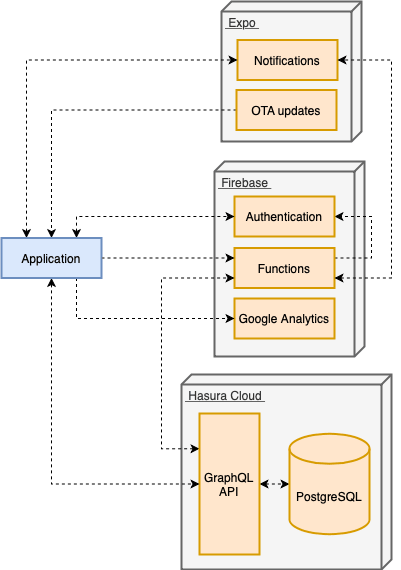
\includegraphics[width=0.5\textwidth]{Images/GameDevelopment/ArchitectureOverview.png}
    \caption{Simplified architectural overview.}
    \label{fig:architecture_overview}
\end{figure}

\subsubsection{The Application}
Hover was developed using React Native and Typescript. The cross-platform framework made it easy to create an application that could be distributed to both iOS and Android using the same codebase. Sometimes there was a minor difference in how the operating systems handled implementation details, which meant we needed to write specific code for both operating systems. However, this was usually not the case, and most of the code functioned very well on both operating systems. Target code to a specific platform is also easily solved in React Native by checking which OS the phone is running.

The application communicates with all three services in the solution. Most of the application data is communicated through the GraphQL API in Hasura, except for authentication information which Firebase is responsible for. Expo provides push notifications and OTA updates. Additionally, the application sends analytics data to Google Analytics.

\subsubsection{Hasura Storage Solution}
Hasura was used as the storage solution in this project. The solution consists of a GraphQL API and a PostgreSQL database where the API is autogenerated based on content in the database. This API and the flexibility of GraphQL allowed us to instantly access the data without needing to develop a custom API. The Hasura solution also included authorization rules where we specified what the users are allowed to fetch and edit. Authentication was solved in Firebase, but a link between Firebase and Hasura updates the user table automatically when new users sign up on Firebase.

\subsubsection{Firebase Backend}
Firebase is used for three main functions in Hover: authentication, back-end provider, and analytics. The authentication solution is, as described above, integrated with Hasura, creating an easy developer experience. It is possible to customize the authentication process to include popular login options such as Facebook and Google. But, in this project, we opted for the standard username and password combination because of privacy limitations.

For doing typical backend operations, we choose to use Firebase Cloud functions. The backend was responsible for tasks that were either too complex for the application or dependent on data updates in the database. A feature in Hasura makes it easy to trigger Firebase functions when the data in the database is updated. Examples of such tasks were validating achievements and challenges and sending push notifications to the user. 

The last Firebase service we used in this project was Google Analytics. This service was set up with the sole purpose of getting usage data from the testing period. Firebase provides a solution for displaying analytics data from your application. The type of data is highly customizable. In our project, this included page views, notification engagement, game events, and more. This data is good content for the next part (Part \ref{part:results}), where we describe the testing results.

\subsubsection{Expo Updates and Notifications}
For deployment and sending push notifications, Expo was used. Using this tool, we can send over-the-air (OTA) software updates of the application without having to rebuild and resubmit the application to App Store and Google Play. OTA updates were a nice feature to have available to deploy bug fixes or critical features quickly. Push notifications are also easily handled using Expo without dealing with the different push notification services for Android and iOS.

\subsection{Summary}
In this chapter, a description of the development process and tools we used has been presented. A general overview of the software architecture and its specific components has also been explained. The next chapter will focus on the mobile application and describe it in further detail.